\documentclass[11pt,a4paper]{article}
\usepackage[margin=2.5cm]{geometry}
\usepackage{booktabs}
\usepackage{listings}
\usepackage{xcolor}
\usepackage{graphicx}
\usepackage{float}

\lstset{
  basicstyle=\ttfamily\small,
  frame=single,
  backgroundcolor=\color{gray!8},
  breaklines=true
}

\title{Labwork 4: Threads}
\author{Yanis Denizot -- 2640051}
\date{\today}

\begin{document}
\maketitle

\section{Implementation}
I copied the grayscale code of labwork 3 and changed the kernel to use 2D blocks. The image
is not flattened anymore: it stays a $(h, w, 3)$ array on the GPU. Each thread computes its
column \texttt{x} and its row \texttt{y}, and checks that it is inside the image.

\begin{lstlisting}[language=Python]
@cuda.jit
def grayscale2d(src, dst):
    x = cuda.threadIdx.x + cuda.blockIdx.x * cuda.blockDim.x
    y = cuda.threadIdx.y + cuda.blockIdx.y * cuda.blockDim.y
    if y < src.shape[0] and x < src.shape[1]:
        g = np.uint8((src[y, x, 0] + src[y, x, 1] + src[y, x, 2]) / 3)
        dst[y, x, 0] = g
        dst[y, x, 1] = g
        dst[y, x, 2] = g

blockSize = (16, 16)
gridSize = ((w + 15) // 16, (h + 15) // 16)
grayscale2d[gridSize, blockSize](devSrc2D, devDst2D)
\end{lstlisting}

The result is the same as the CPU version. I ran it on Google Colab (Tesla T4) with the same
image as labwork 3 ($471 \times 651$ pixels). The CPU loop takes 0.431 s. For each block
size, the GPU time is the average of 100 launches, and I compare with the 1D kernel using the
same number of threads per block.

\section{Results}

\begin{table}[H]
\centering
\begin{tabular}{lrrrr}
\toprule
Block & 1D ($\mu$s) & 2D ($\mu$s) & 1D speedup & 2D speedup \\
\midrule
$8 \times 8$   & 79.2 & 80.9 & 5450 & 5336 \\
$16 \times 8$  & 78.3 & 82.2 & 5512 & 5247 \\
$16 \times 16$ & 78.8 & 80.9 & 5475 & 5336 \\
$32 \times 16$ & 78.4 & 83.1 & 5504 & 5189 \\
$32 \times 32$ & 87.9 & 90.0 & 4907 & 4792 \\
\bottomrule
\end{tabular}
\end{table}

\begin{figure}[H]
\centering
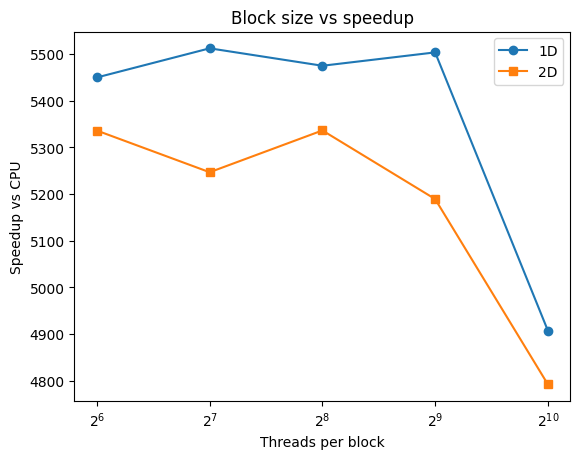
\includegraphics[width=0.65\textwidth]{blocksize_vs_speedup.png}
\end{figure}

The speedup is around 5000 for both, but 2D is a bit slower than 1D (2 to 6\%). For
grayscale each pixel is computed alone, so 2D does not really help. It is even a little
slower because the image size is not a multiple of the block size, so some threads on the
borders do nothing (2.7\% with $16 \times 16$), and each thread computes two indices instead
of one. Like in labwork 3, 1024 threads per block is the slowest.

\section{Exercises}

\textbf{Exercise 1.} $16 \times 16$. With $8 \times 8$ (64 threads), the SM can only take
8 blocks, so $8 \times 64 = 512$ threads, half of the SM. $32 \times 32$ is 1024 threads, more
than the 512 threads/block limit. $16 \times 16$ gives 256 threads, so 4 blocks fill the SM
with 1024 threads.

\textbf{Exercise 2.} 512 threads/block. $3 \times 512 = 1536$, so the SM is full. With 128 or
256, the 4 blocks limit gives only 512 or 1024 threads. With 1024, only one block fits
(two would be 2048).

\textbf{Exercise 3.} $2000 / 512 = 3.9$, so we need 4 blocks, which gives
$4 \times 512 = 2048$ threads. The last 48 threads do nothing, so the kernel needs a check
\texttt{if tid < 2000}.

\end{document}
